\documentclass[border=.2cm]{standalone}
\usepackage{tikz}
\usepackage{amsmath}

\begin{document}

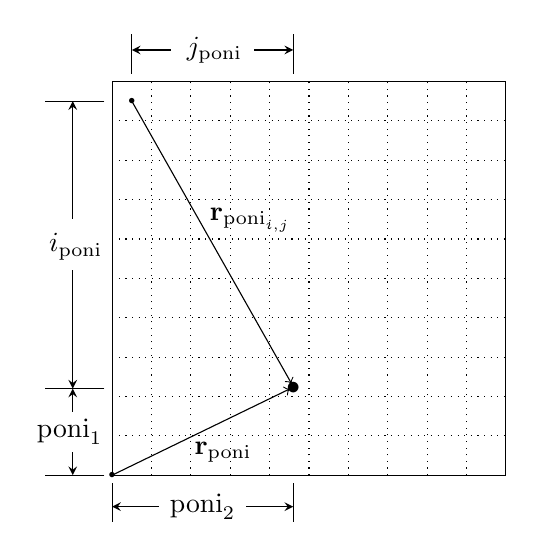
\begin{tikzpicture}
    \def \length {5};
    \foreach \ii in {0, 5} {
        \draw (\ii, 0) --++ (0, \length);
        \draw (0, \ii) --++ (\length, 0);
    }
    \foreach \ii in {1, ..., 9} {
        \draw[dotted] (0.5 * \ii, 0) --++ (0, \length)
                      (0, 0.5 * \ii) --++ (\length, 0);
    }
    \def \x{2.3}; \def \y{1.1};
    \draw[->] (0, 0) node[scale=0.5] {$\bullet$} -- (\x*.98, \y*.995) node[midway, right, below,xshift=8] {$\mathbf{r}_\text{poni}$};
    \draw[->] (0.25, \length-0.25) node[scale=0.5] {$\bullet$} -- (\x*.99, \y*1.06) node[midway, right, above, xshift=14] {$\mathbf{r}_{\text{poni}_{i,j}}$};
    \node at (\x, \y) {$\bullet$};
    \foreach \ii in {0, \y, \length-0.25} {
        \draw (-.1, \ii) --++ (-.75, 0);
    }
    \draw[stealth-] (-0.5, 0) --++ (0, .3);
    \draw[stealth-] (-0.5, \y) --++ (0, -.3);
    \node[anchor=east] at (0, 0.5*\y) {$\text{poni}_1$};

    \draw[stealth-] (-0.5, \y) --++ (0, 1.5);
    \draw[stealth-] (-0.5, \length-.25) --++ (0, -1.5);
    \node[anchor=east] at (0, 2.9) {$i_\text{poni}$};

    \foreach \ii in {0, \x} {
        \draw (\ii, -.1) --++ (0, -.5);
    }
    \node at (0.5*\x, -.4) {$\text{poni}_2$};
    \draw[stealth-] (0, -.4) --++ (.6, 0);
    \draw[stealth-] (\x, -.4) --++ (-.6, 0);

    \foreach \ii in {0.25, \x} {
        \draw (\ii, 5.1) --++ (0, .5);
    }
    \node at (1.3, 5.4) {$j_\text{poni}$};
    \draw[stealth-] (0.25, 5.4) --++ (.5, 0);
    \draw[stealth-] (\x, 5.4) --++ (-.5, 0);
\end{tikzpicture}

\end{document}